\documentclass[12pt,onecolumn]{article}
\usepackage[utf8]{inputenc} % UTF8 input encoding
\usepackage[T2A]{fontenc}   % T2A font encoding for Cyrillic script
\usepackage[russian]{babel} % Russian language support
\usepackage{listings}
\usepackage{float}
\usepackage{mathtools}
\everymath{\displaystyle}
\usepackage{listings} 
\usepackage[usenames]{color}
\usepackage{hyperref}
\usepackage{geometry}
\usepackage{verbatim}
\usepackage{framed}
\usepackage{amsmath}
\usepackage{tcolorbox}
\usepackage{pdfpages}
\usepackage{graphicx}
\usepackage[dvipsnames]{xcolor}
\usepackage{svg}
\usepackage{tabularx}
\usepackage{multirow}
\usepackage{graphicx}
\usepackage[smartEllipses]{markdown}
\newcommand{\nparagraph}[1]{\paragraph{#1}\mbox{}\\}
\geometry{
  a4paper,
  top=20mm, 
  right=20mm, 
  bottom=20mm, 
  left=25mm
}
\lstdefinestyle{listing}{ 
  basicstyle=\small\ttfamily,
  commentstyle=\color{cyan},
  stringstyle=\color{magenta}\ttfamily,
  keywordstyle=\color{blue},
  numbers=left,
  numberstyle=\scriptsize,
  numbersep=5pt,
  frame=single,
  breaklines=true,
  breakatwhitespace=true,
  showstringspaces=false,
  tabsize=4,
  inputencoding=utf8,
  extendedchars=true,
  literate={ε}{{$\epsilon$}}1 {→}{{$\rightarrow$}}1
}

% Define a command to highlight text with a blue background
\newcommand{\hlb}[1]{
  \colorbox{Cyan}{#1}
}

% Define a command to highlight text with a lime green background
\newcommand{\hlg}[1]{
  \colorbox{LimeGreen}{#1}
}

% Define a command to highlight text with a pink background
\newcommand{\hlp}[1]{
  \colorbox{Lavender}{#1}
}

% Define a command to highlight text with a red background
\newcommand{\hlr}[1]{
  \colorbox{Salmon}{#1}
}

% Define a command to highlight text with a yellow background
\newcommand{\hly}[1]{
  \colorbox{Goldenrod}{#1}
}

% Define a command to highlight text with a orange background
\newcommand{\hlo}[1]{
  \colorbox{BurntOrange}{#1}
}

% Command: \chtb
% Description: Creates a centered table with two columns, where the first column contains the expression specified by the argument #3, and the second column contains the expression specified by the argument #4. The table width is determined by the argument #1.
% Parameters:
%   - #1: The width of the table (e.g., \textwidth, 0.8\linewidth)
%   - #2: The title of the table
%   - #3: The expression to be displayed in the first column
%   - #4: The expression to be displayed in the second column
\newcommand{\chtb}[4]{
  \begin{center}
    \textbf{#2}
  \end{center}
  \begin{center}
    \begin{tabularx}{#1}{X|X}
    $\begin{aligned}
          #3
      \end{aligned}$ &
    \begin{minipage}{1em}
      $\Rightarrow$
    \end{minipage}
    $\begin{aligned}
         #4
      \end{aligned}$
    \end{tabularx}
  \end{center}
}



\begin{document}
\setcounter{tocdepth}{4}
\begin{center}
    Федеральное государственное автономное образовательное учреждение высшего образования "Национальный Исследовательский Университет ИТМО"\\
    Мегафакультет Компьютерных Технологий и Управления\\
    Факультет Программной Инженерии и Компьютерной Техники \\
    
\includegraphics[scale=0.3]{image/itmo.jpg} % нужно закинуть картинку логтипа в папку с отчетом
\end{center}
\vspace{1cm}


\begin{center}
    \large \textbf{Вариант №5}\\
    \textbf{Задание}\\
    по дисциплине\\
    \textbf{'Разработка компиляторов'}
\end{center}

\vspace{2cm}

\begin{flushright}
    Выполнил Студент  группы P33102\\
    \textbf{Лапин Алексей Александрович}\\
    Преподаватель: \\
    \textbf{Лаздин Артур Вячеславович}\\
\end{flushright}

\vspace{9cm}
\begin{center}
    г. Санкт-Петербург\\
    2024г.
\end{center}
\pagestyle{empty}


\section*{Задание}
Разработать язык программирования, который должен реализовать следующие компоненты:

\begin{enumerate}
    \item Присваивание (оператор или операция), арифметические и логические операции.
    \item Ветвление, включая вариант факультативного else.
    \item Цикл while.
    \item Поддержка целочисленного и логического типа данных.
    \item Многострочные комментарии в стиле Си-подобных языков.
\end{enumerate}

Что добавит баллы:
\begin{enumerate}
    \item Вместо ветвление if [then] else конструируется
          оператор if elif [elif]+ else
    \item Вместо цикла while (или в дополнение к нему) конструируется цикл for.
\end{enumerate}

\section{Ход работы}
Сделал лексический анализатор грамматики с помощью библиотеки FLEX.
\lstinputlisting[style=listing, language=C]{../lexer.l}
Сделал синтаксический анализатор грамматики с помощью библиотеки BISON.
\lstinputlisting[style=listing, language=C]{../parser.y}

\section{Проверка соответсвия требованиям}
\subsection{Присваивание (оператор или операция)}
\begin{figure}[H]
    \centering
    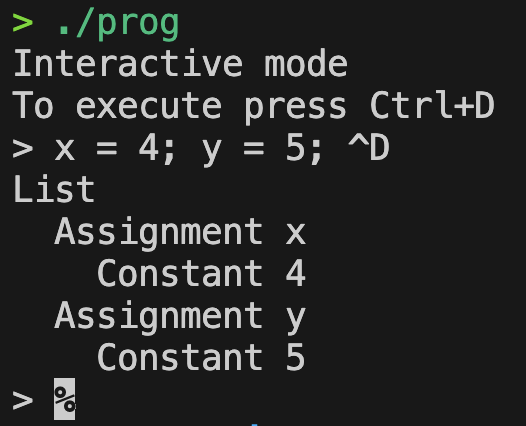
\includegraphics[width=0.5\textwidth]{image/asgn.png}
    \caption{Присваивание}
\end{figure}
\textbf{out.S:}
\begin{verbatim}
    jal x1, MAIN
    x:
    data 0 * 1
    y:
    data 0 * 1
    MAIN:
    li x1, 4
    sw x0, 1, x1
    li x1, 5
    sw x0, 2, x1
    ebreak
\end{verbatim}
\subsection{Арифметические и логические операции. Ветвление, включая вариант факультативного elif.Поддержка целочисленного и логического типа данных.Многострочные комментарии в стиле Си-подобных языков.}
\textbf{Программа:}
\lstinputlisting[style=listing]{../tests/2.t}
\textbf{tree:}
\begin{verbatim}
List
Assignment x
    Constant 4
List
    Assignment y
    Constant 0
    List
    Assignment z
        Constant 0
    If
        Symbol y
        Assignment z
        Constant 1
        If
        Comparison ==
            Symbol x
            Constant 4
        Assignment z
            Constant 2
        Assignment z
            Constant 3  
\end{verbatim}
\textbf{out.S:}
\begin{verbatim}
jal x1, MAIN
x:
data 0 * 1
y:
data 0 * 1
z:
data 0 * 1
MAIN:
li x1, 4
sw x0, 1, x1
li x1, 0
sw x0, 2, x1
li x1, 0
sw x0, 3, x1
lw x2, x0, 2
beq x2, x0, ELSE0
li x1, 1
sw x0, 3, x1
jal x1, ENDIF0
ELSE0:
lw x2, x0, 1
li x3, 4
seq x2, x2, x3
beq x2, x0, ELSE1
li x1, 2
sw x0, 3, x1
jal x1, ENDIF1
ELSE1:
li x1, 3
sw x0, 3, x1
ENDIF1:
ENDIF0:
ebreak
\end{verbatim}
\begin{figure}[H]
    \centering
    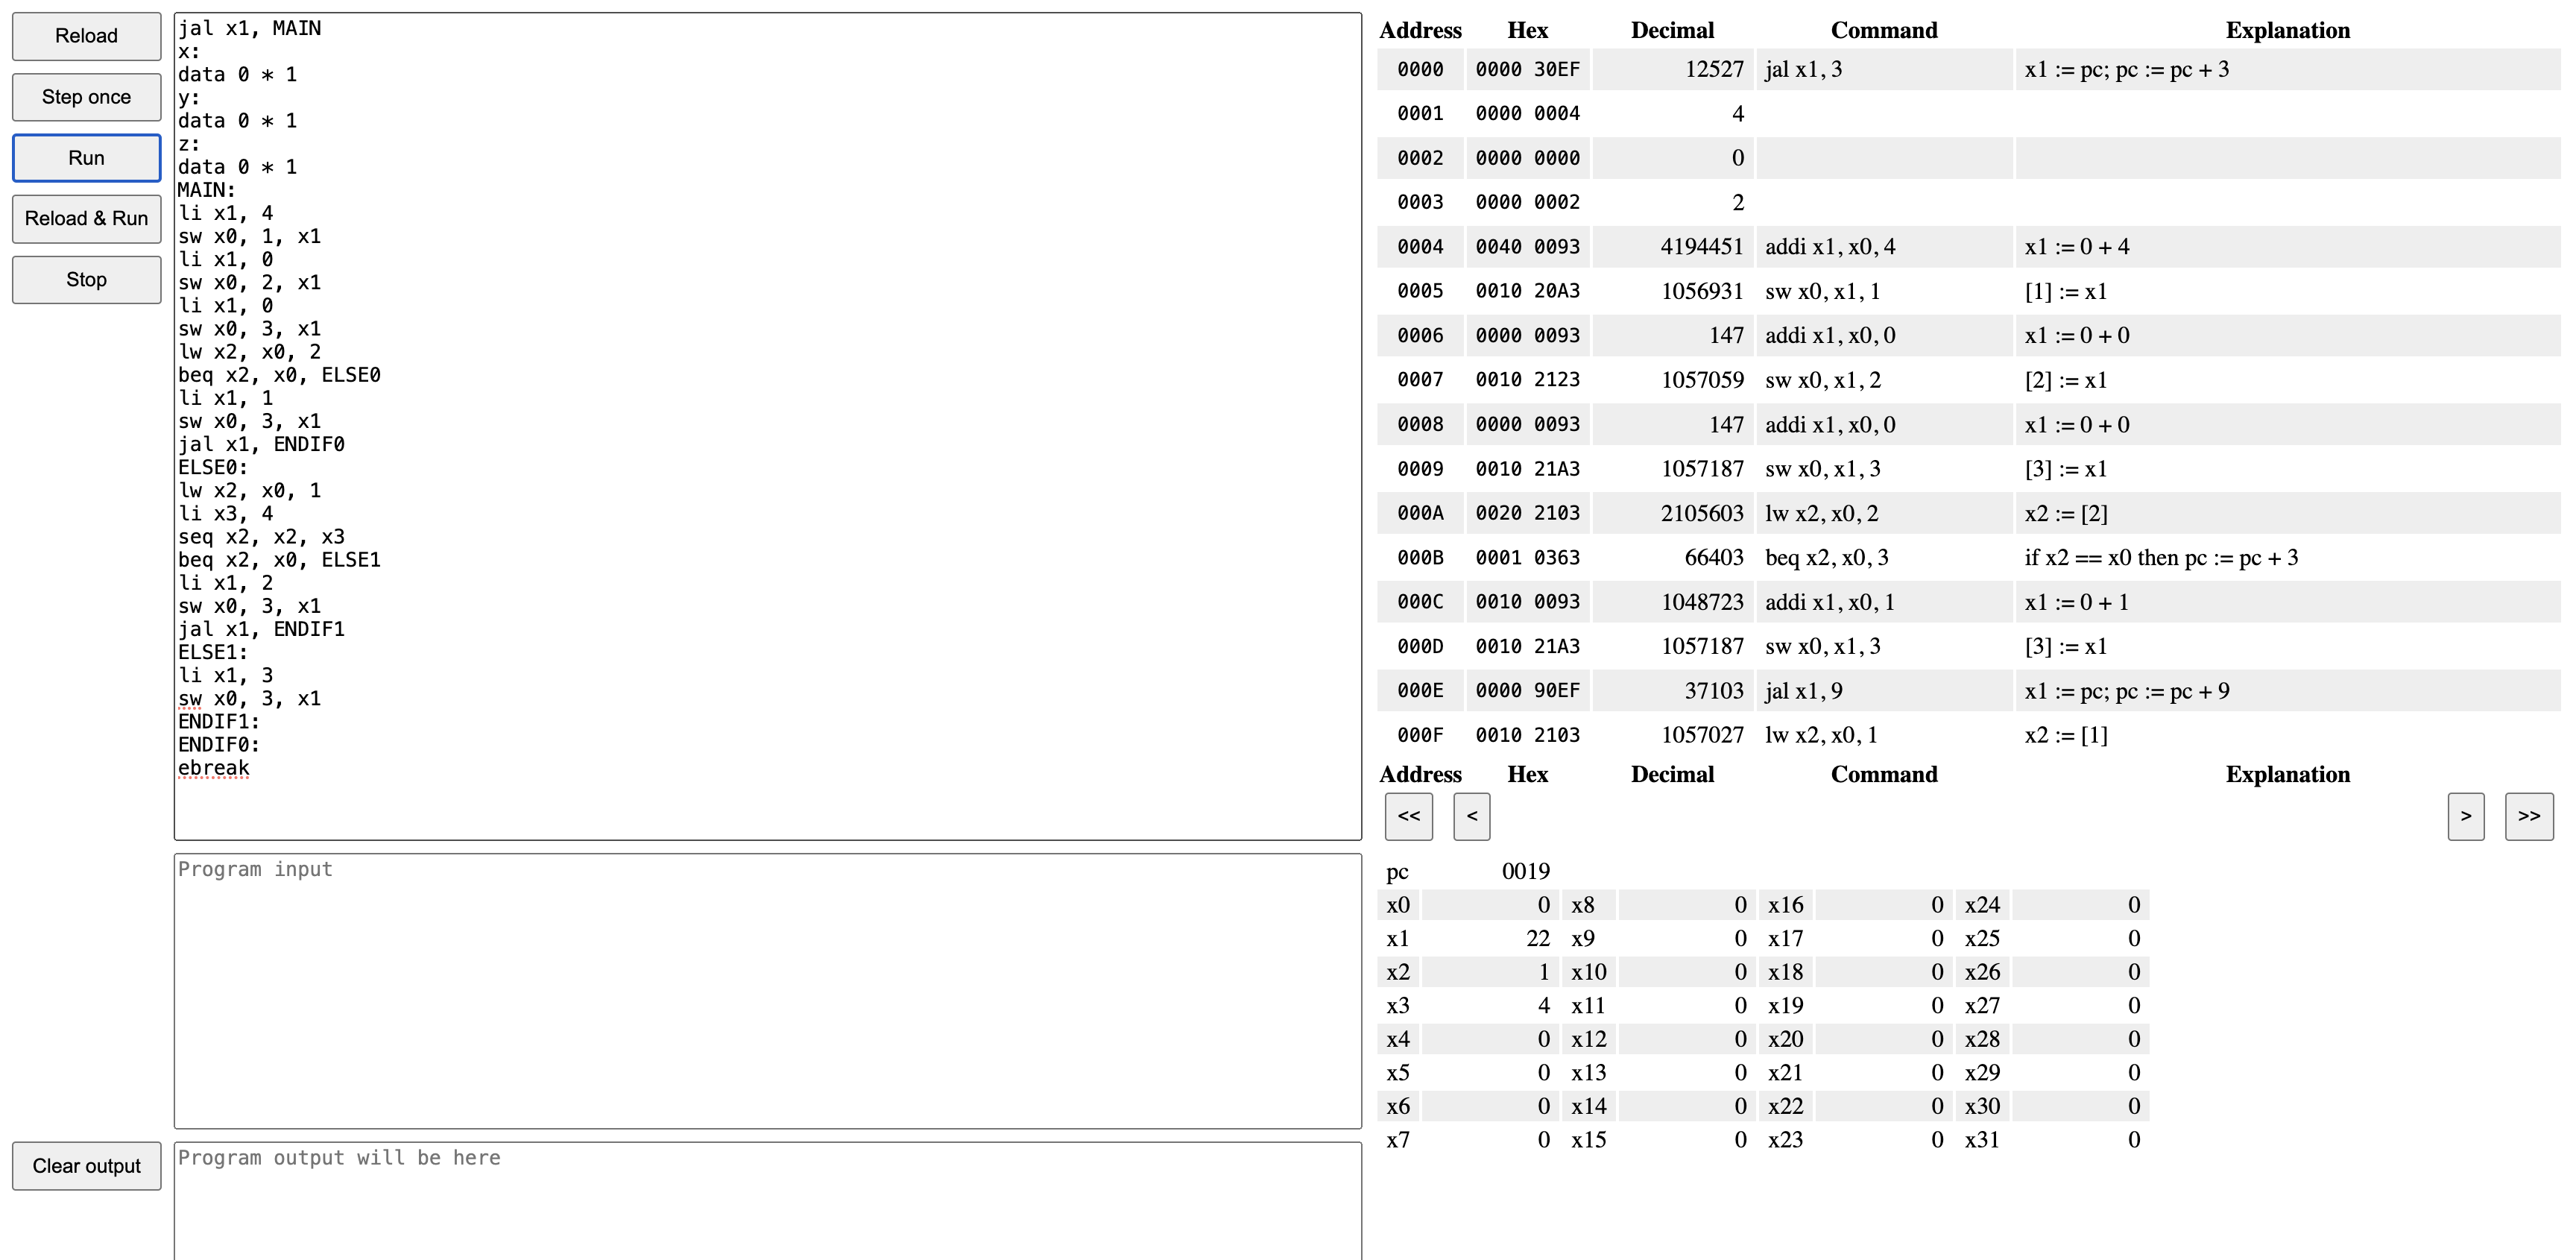
\includegraphics[width=\textwidth]{image/out2.png}
    \caption{Программа}
\end{figure}

\subsection{Оператор For}
\textbf{Программа:}
\lstinputlisting[style=listing]{../tests/3.t}
\textbf{tree:}
\begin{verbatim}
List
Assignment x
    Constant 4
List
    Assignment y
    Constant 32
    For
    Assignment i
        Constant 1
    Comparison <
        Symbol i
        Constant 5
    Assignment i
        Operator +
        Symbol i
        Constant 1
    List
        Assignment x
        Operator *
            Symbol x
            Symbol i
        Assignment y
        Operator /
            Symbol y
            Constant 2
\end{verbatim}
\textbf{out.S:}
\begin{verbatim}
jal x1, MAIN
i:
data 0 * 1
x:
data 0 * 1
y:
data 0 * 1
MAIN:
li x1, 4
sw x0, 2, x1
li x1, 32
sw x0, 3, x1
li x1, 1
sw x0, 1, x1
WHILE0:
lw x2, x0, 1
li x3, 5
slt x2, x2, x3
beq x2, x0, ENDWHILE0
lw x1, x0, 2
lw x2, x0, 1
mul x1, x1, x2
sw x0, 2, x1
lw x1, x0, 3
li x2, 2
div x1, x1, x2
sw x0, 3, x1
lw x1, x0, 1
li x2, 1
add x1, x1, x2
sw x0, 1, x1
jal x1, WHILE0
ENDWHILE0:
ebreak
\end{verbatim}

\begin{figure}[H]
    \centering
    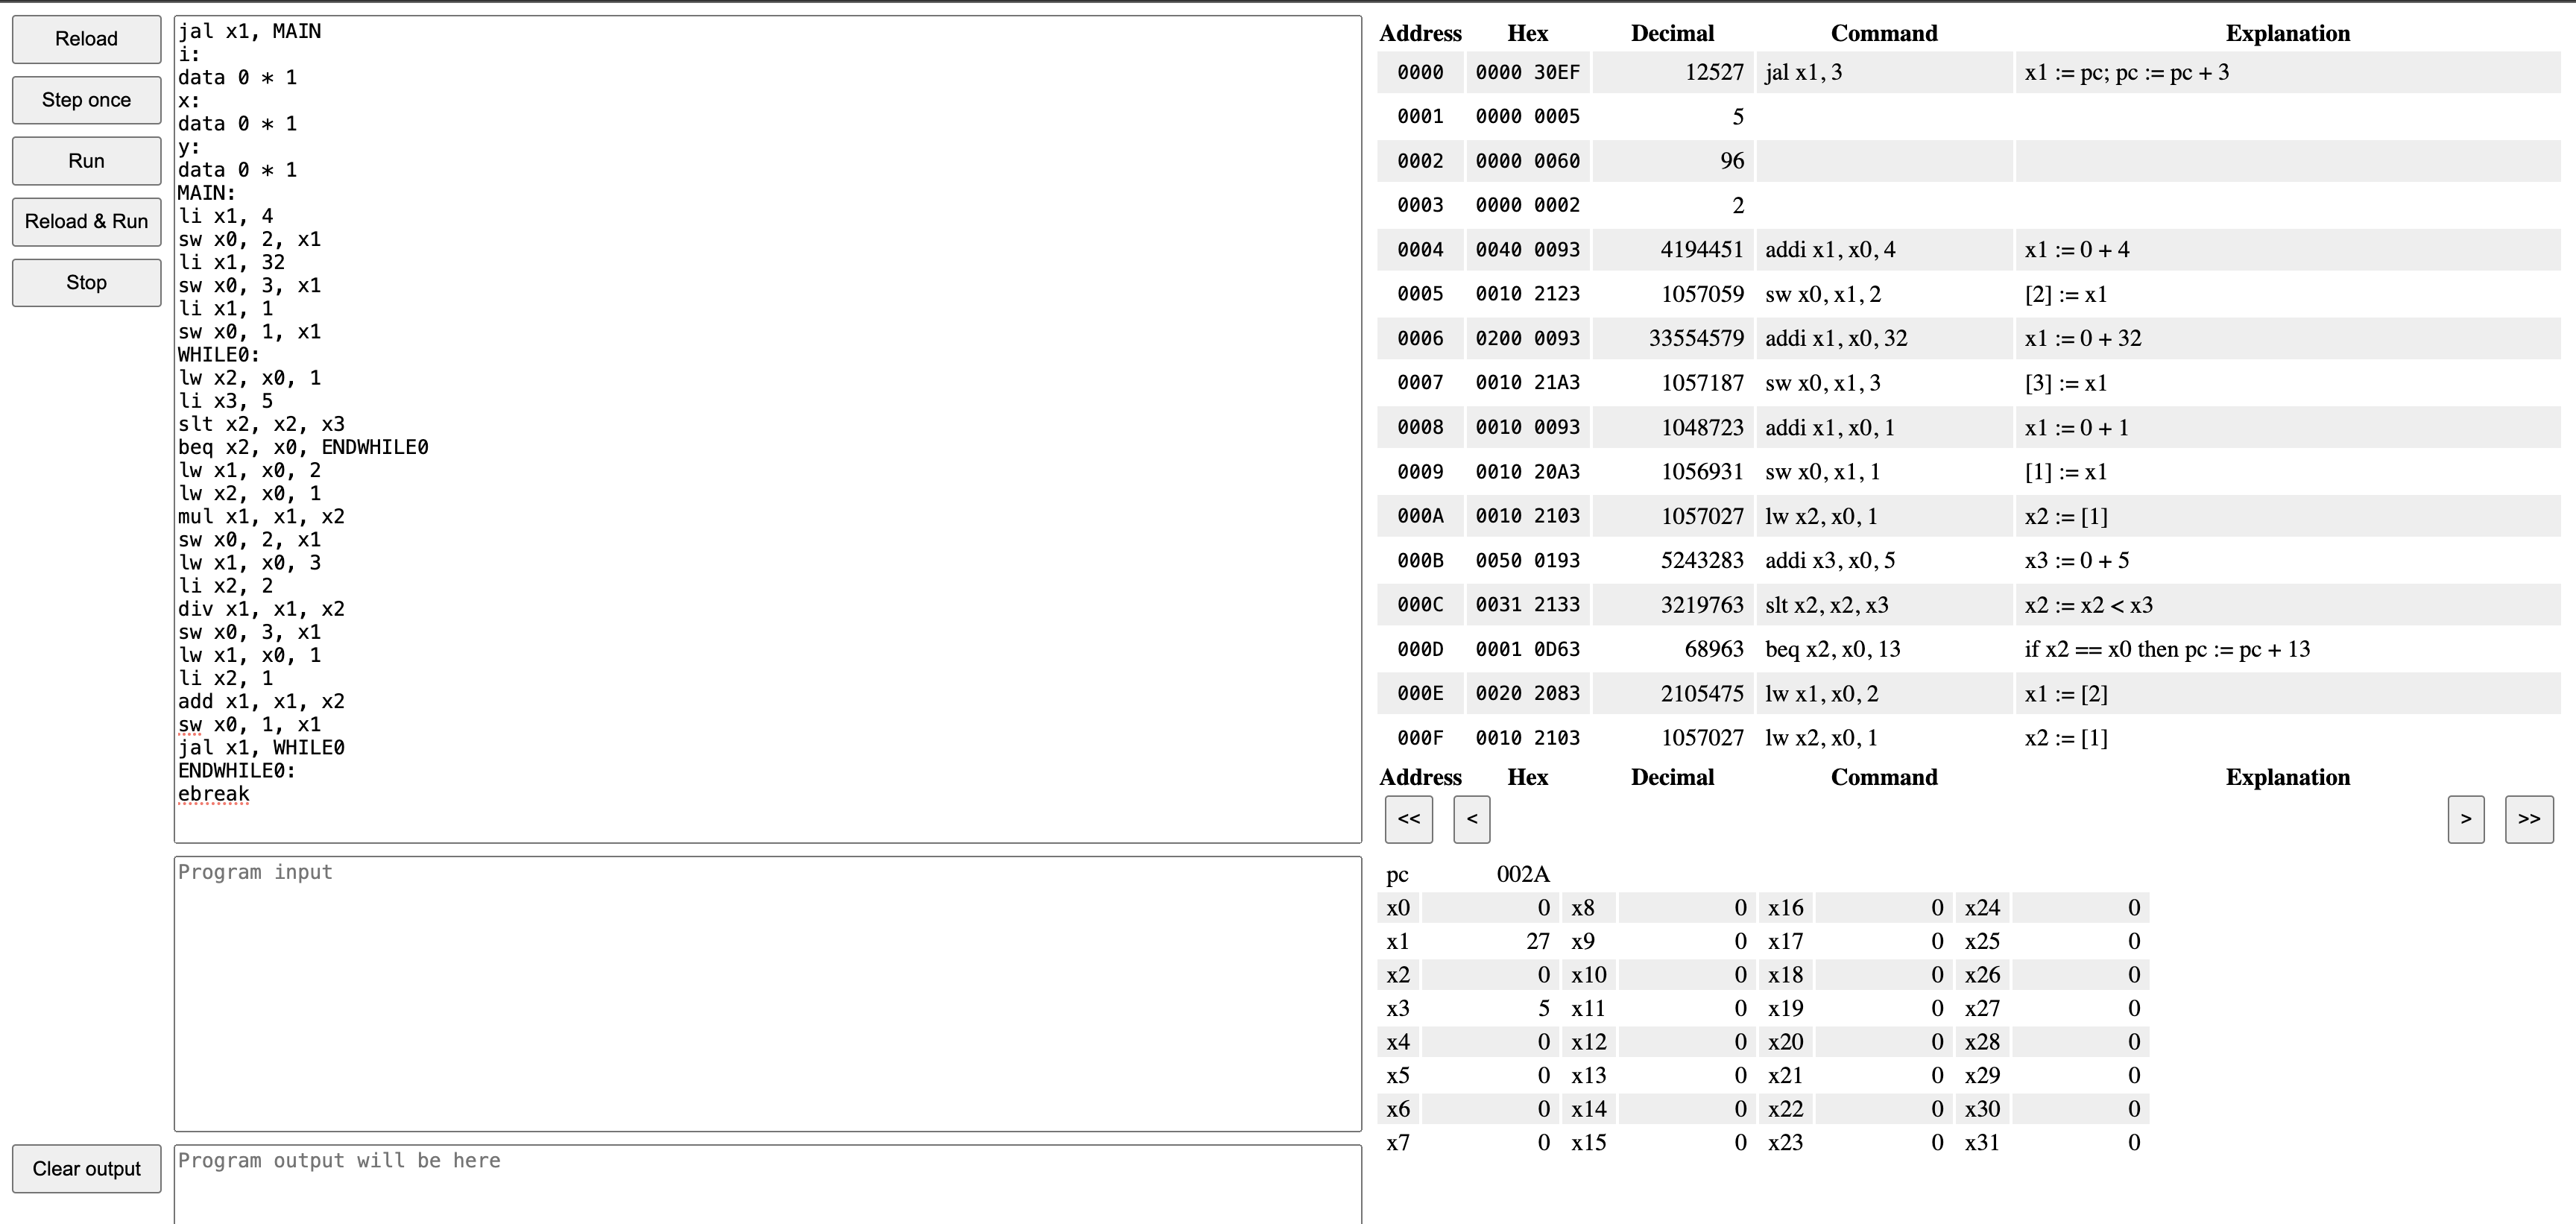
\includegraphics[width=\textwidth]{image/out3.png}
    \caption{Программа}
\end{figure}


\subsection{Оператор While}
\textbf{Программа:}
\lstinputlisting[style=listing]{../tests/3.t}
\textbf{tree:}
\begin{verbatim}
List
  Assignment x
    Constant 2
  While
    Comparison <=
      Symbol x
      Constant 10
    If
      Comparison ==
        Symbol x
        Constant 4
      Assignment x
        Operator +
          Symbol x
          Constant 2
      Assignment x
        Operator +
          Symbol x
          Constant 1

\end{verbatim}
\begin{verbatim}
jal x1, MAIN
x:
data 0 * 1
MAIN:
li x1, 2
sw x0, 1, x1
WHILE0:
lw x2, x0, 1
li x3, 10
seq x4, x2, x3
slt x5, x2, x3
or x2, x4, x5
beq x2, x0, ENDWHILE0
lw x2, x0, 1
li x3, 4
seq x2, x2, x3
beq x2, x0, ELSE0
lw x1, x0, 1
li x2, 2
add x1, x1, x2
sw x0, 1, x1
jal x1, ENDIF0
ELSE0:
lw x1, x0, 1
li x2, 1
add x1, x1, x2
sw x0, 1, x1
ENDIF0:
jal x1, WHILE0
ENDWHILE0:
ebreak
\end{verbatim}


\begin{figure}[H]
    \centering
    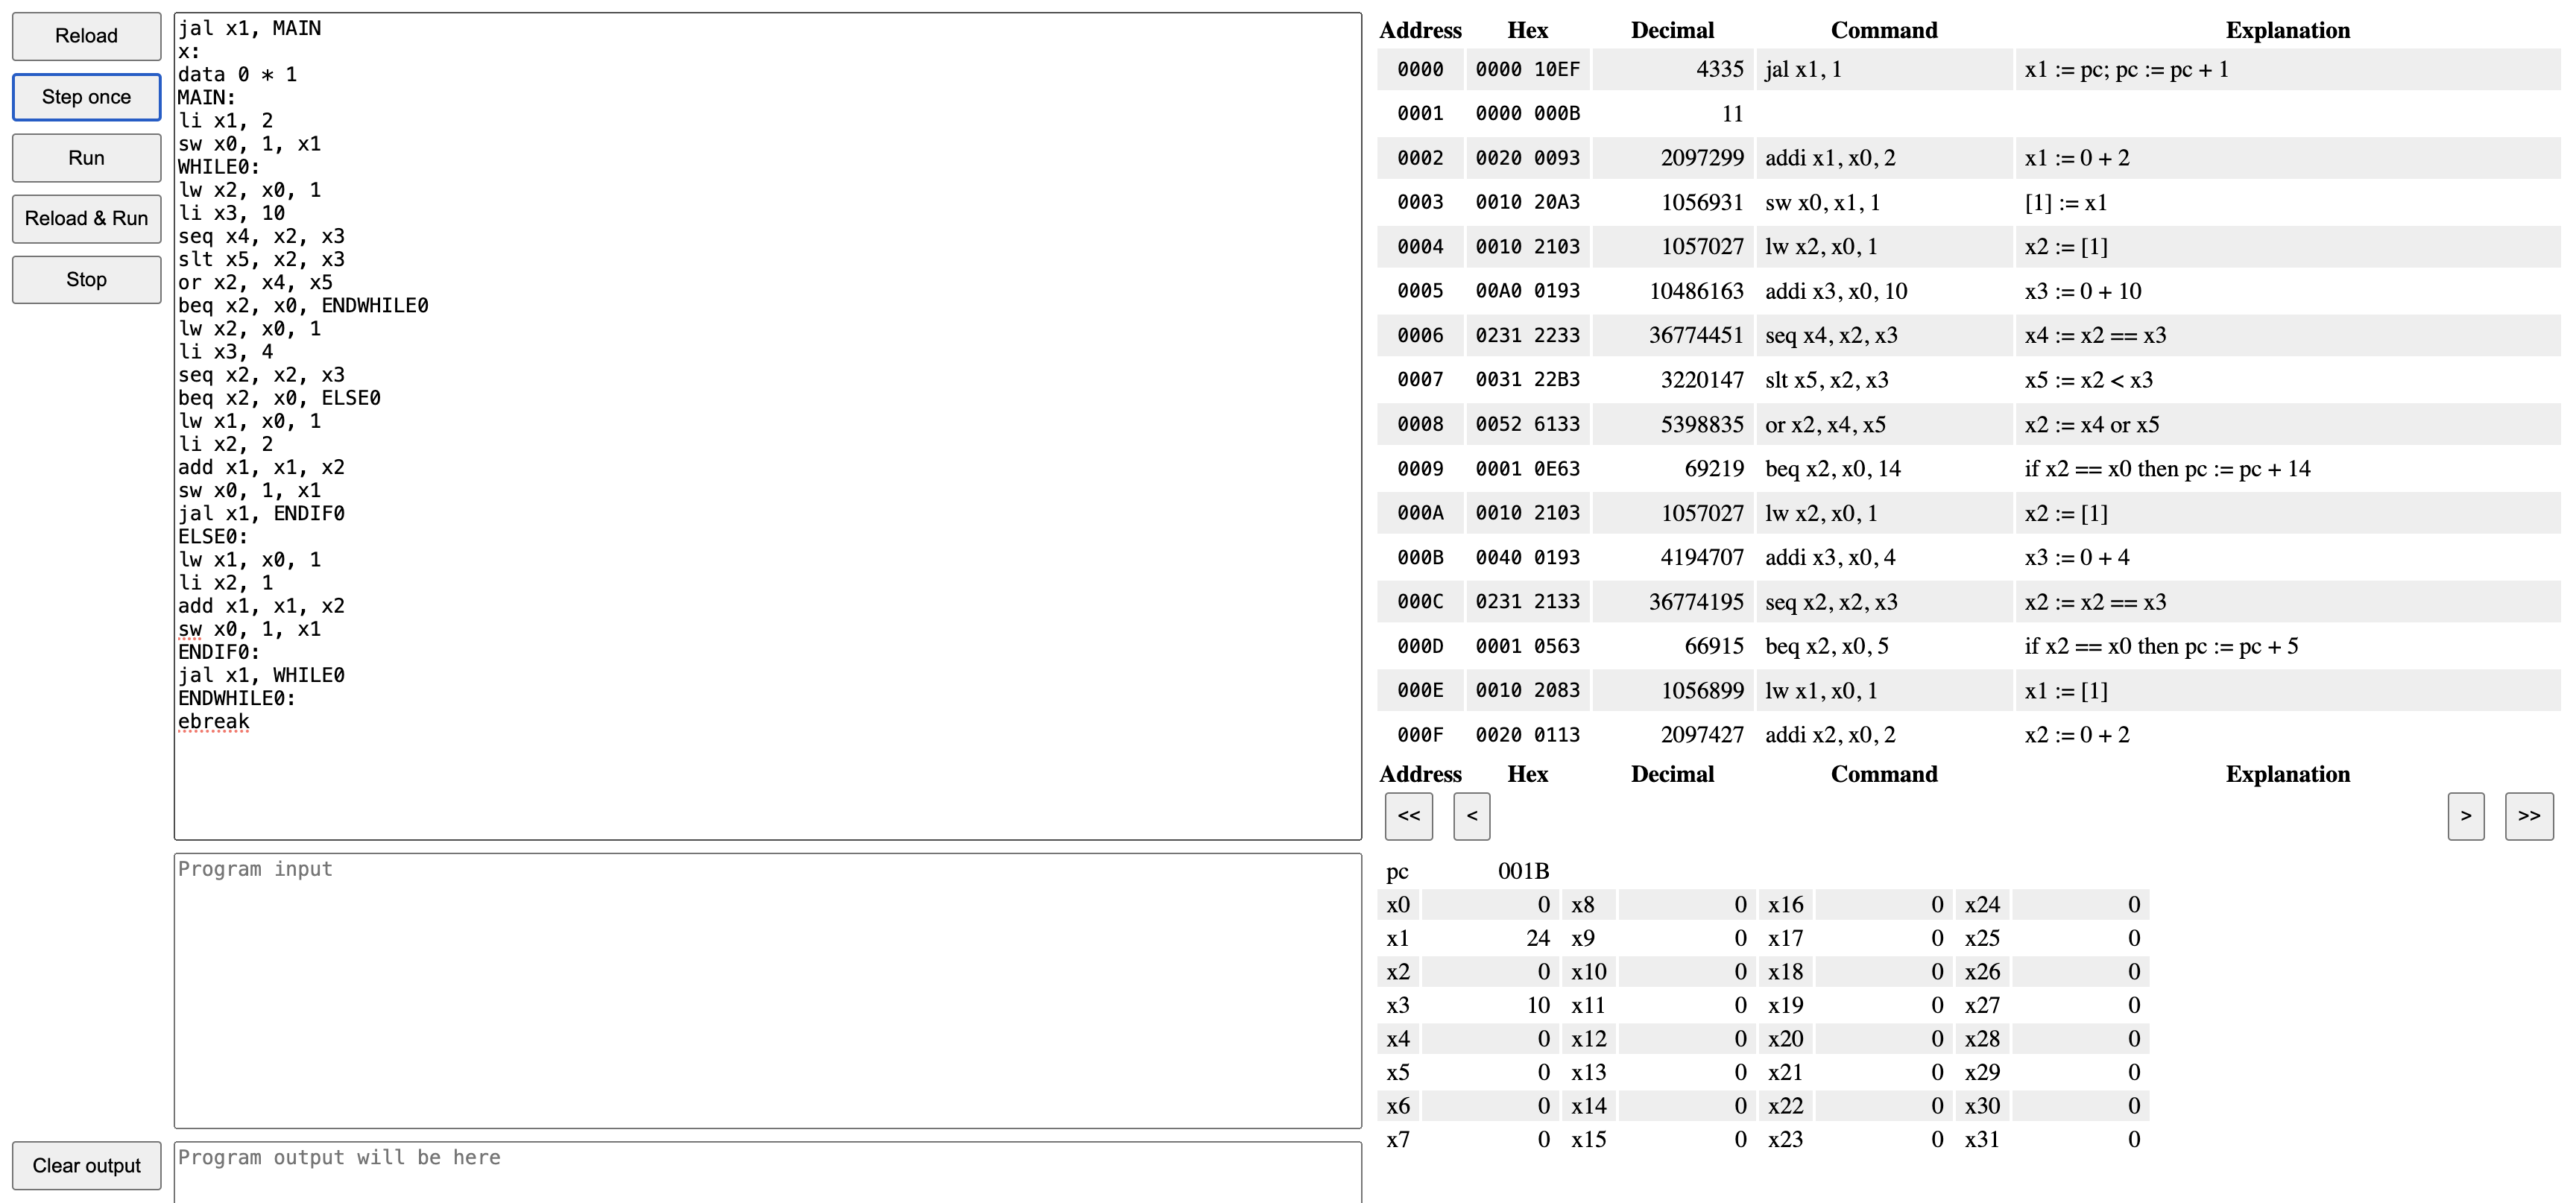
\includegraphics[width=\textwidth]{image/out4.png}
    \caption{Программа}
\end{figure}


\section{Обработка ошибок}
\begin{figure}[H]
    \centering
    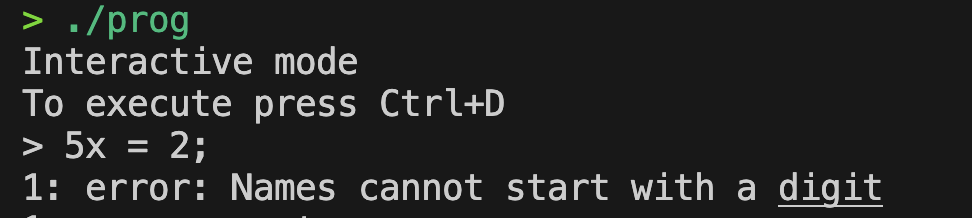
\includegraphics[width=0.5\textwidth]{image/error1.png}
\end{figure}
\begin{figure}[H]
    \centering
    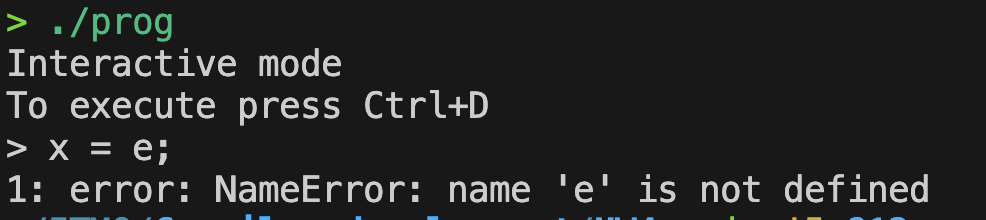
\includegraphics[width=0.5\textwidth]{image/error2.png}
\end{figure}
\begin{figure}[H]
    \centering
    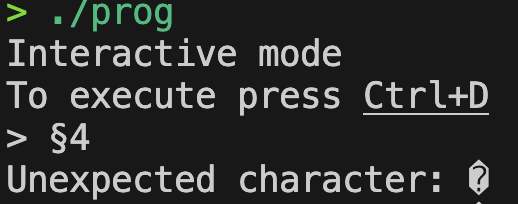
\includegraphics[width=0.5\textwidth]{image/error3.png}
\end{figure}

\end{document}